% ============================================================
% Rapport-Critique — Critical Review of Rapport 2
% An Agentic Framework for IaC Misconfiguration Analysis
% and Remediation
%
% Ahmedou Yahye Kheyri
% Supervised by: Hala Bezine
% Faculté des Sciences de Sfax --- Master MRSI
% 2025--2026
% ============================================================

\documentclass[11pt, a4paper]{report}

% ---- Encoding & Language ----
\usepackage[utf8]{inputenc}
\usepackage[T1]{fontenc}
\usepackage[english]{babel}

% ---- Layout ----
\usepackage[top=2.5cm, bottom=2.5cm, left=3cm, right=2.5cm]{geometry}
\usepackage{setspace}
\onehalfspacing
\setlength{\parindent}{1.2em}
\setlength{\parskip}{0.4em}
\setlength{\headheight}{14pt}

% ---- Fonts ----
\usepackage{lmodern}
\usepackage{microtype}

% ---- Math ----
\usepackage{amsmath}
\usepackage{amssymb}

% ---- Graphics & Tables ----
\usepackage{graphicx}
\usepackage{float}
\usepackage{booktabs}
\usepackage{tabularx}
\usepackage{longtable}
\usepackage{array}
\usepackage[table,xcdraw]{xcolor}

% ---- Code Listings ----
\usepackage{listings}
\usepackage{lstautogobble}
\definecolor{codegray}{rgb}{0.5,0.5,0.5}
\definecolor{backcolour}{rgb}{0.97,0.97,0.97}
\lstset{
  backgroundcolor=\color{backcolour},
  basicstyle=\ttfamily\small,
  breakatwhitespace=false, breaklines=true,
  captionpos=b, keepspaces=true,
  numbers=left, numbersep=6pt,
  numberstyle=\tiny\color{codegray},
  showspaces=false, showstringspaces=false, showtabs=false,
  tabsize=2, frame=single, rulecolor=\color{gray!40},
  autogobble=true
}

% ---- TikZ for timeline ----
\usepackage{tikz}
\usetikzlibrary{shapes.geometric, arrows.meta, positioning, fit, calc}

% ---- Colors ----
\definecolor{critblue}{RGB}{40,70,140}
\definecolor{critred}{RGB}{180,40,40}
\definecolor{critgreen}{RGB}{40,140,70}
\definecolor{critorange}{RGB}{200,110,30}

% ---- Hyperlinks ----
\usepackage[
  colorlinks=true,
  linkcolor=blue!70!black,
  citecolor=blue!60!black,
  urlcolor=blue!80!black
]{hyperref}
\usepackage{url}

% ---- Bibliography ----
\usepackage[numbers,sort&compress]{natbib}
\bibliographystyle{IEEEtranN}

% ---- Boxes ----
\usepackage{tcolorbox}
\tcbuselibrary{breakable, skins}

\newtcolorbox{gradebox}[2][]{
  colback=#2!6!white, colframe=#2!55!black,
  fonttitle=\bfseries, title={#1},
  breakable, enhanced
}

\newtcolorbox{findingbox}[1][]{
  colback=yellow!8!white, colframe=orange!55!black,
  fonttitle=\bfseries, title={#1},
  breakable, enhanced
}

% ---- Caption ----
\usepackage[font=small,labelfont=bf]{caption}

% ---- Headers & Footers ----
\usepackage{fancyhdr}
\pagestyle{fancy}
\fancyhf{}
\fancyhead[L]{\small\leftmark}
\fancyhead[R]{\small\thepage}
\fancyfoot[C]{\small Rapport-Critique --- Ahmedou Yahye Kheyri}
\renewcommand{\headrulewidth}{0.4pt}

% ---- Chapter style ----
\usepackage{titlesec}
\titleformat{\chapter}[display]
  {\normalfont\huge\bfseries\color{critblue}}
  {\chaptertitlename\ \thechapter}{16pt}{\Huge}
\titlespacing*{\chapter}{0pt}{-10pt}{20pt}

% ============================================================
\begin{document}
% ============================================================

% ---- Title Page ----
\begin{titlepage}
  \centering

  \vspace*{2.5cm}
  {\small Ministère de l'Enseignement Supérieur, de la Recherche Scientifique
   et de la Technologie}\\[4pt]
  {\small Université de Sfax \enspace\textbar\enspace Faculté des Sciences de Sfax}\\[4pt]
  {\small Département d'Informatique \enspace\textbar\enspace Master MRSI}

  \vspace{2.5cm}
  \noindent\rule{\linewidth}{0.6pt}\\[0.8cm]

  {\LARGE\bfseries\color{critblue}
    Critical Review of Rapport~2\\[6pt]
    An Honest Assessment and Redirection\\[4pt]
    Toward Rapport~4
  }\\[0.8cm]

  \noindent\rule{\linewidth}{0.6pt}

  \vspace{0.6cm}
  {\normalsize\itshape Technical Report --- Rapport-Critique}

  \vspace{3cm}
  \begin{minipage}[t]{0.45\textwidth}
    \raggedright
    {\small\bfseries Prepared by}\\[4pt]
    {\normalsize Ahmedou Yahye Kheyri}
  \end{minipage}
  \hfill
  \begin{minipage}[t]{0.45\textwidth}
    \raggedleft
    {\small\bfseries Supervised by}\\[4pt]
    {\normalsize Pr.\ Hala Bezine}
  \end{minipage}

  \vfill
  {\small Academic Year 2025--2026 \enspace\textbar\enspace April 2026}
  \vspace{1cm}
\end{titlepage}

% ---- Abstract ----
\chapter*{Abstract}
\addcontentsline{toc}{chapter}{Abstract}

This document is an internal critical review of Rapport~2 of the thesis
\emph{An Agentic Framework for Infrastructure as Code (IaC) Misconfiguration
Analysis and Remediation}. It was written after a bibliographic survey of
benchmarks and IaC security literature published between April~2025 and
April~2026, and is intended to redirect the work toward Rapport~4 on a
stronger empirical and positioning footing.

The review is deliberately blunt. Three of the six contributions claimed in
Rapport~2 are reclassified as engineering deliverables or negative baselines
rather than research contributions. Five of the eighteen evaluation metrics
are either non-computable on the current backend, trivially saturated, or
conceptually misapplied; concrete replacements are proposed. A benchmark
landscape comparison places the framework's target niche --- agentic IaC
security remediation with independent tool-based validation --- in context of
recent benchmarks published in 2025 and early 2026 (PatchEval~\citep{lyu2024patcheval},
AutoPatchBench~\citep{autopatchbench2025}, SEC-bench~\citep{secbench2025},
SecRepoBench~\citep{secrepobench2025}, IntelliSA~\citep{intellisa2026},
IaC-Eval~\citep{kon2024iaceval}, Multi-IaC-Eval~\citep{multi2025iaceval}).
The niche is confirmed to be genuinely unoccupied, but Rapport~2 has not yet
demonstrated that the framework occupies it; Rapport~4 must close this gap.

\bigskip
\noindent\textbf{Keywords:} Self-critique, Research validity, IaC security,
Benchmark survey, Rapport~4 planning.

% ---- TOC ----
\tableofcontents

% ============================================================
\chapter{Purpose and Scope}
% ============================================================

\section{Why this document exists}

Rapport~2 was submitted in April~2026 as the main technical report of the
thesis. It describes the framework architecture, a 27-smell evaluation
dataset, eighteen evaluation metrics, and a Config~A baseline
($\text{Macro-F1} = 0.082$ for Checkov alone). Between Rapport~2 and the
present date, the following things have happened:

\begin{itemize}
  \item Rapport~3 has been drafted, documenting a 33{,}667-record IaC security
        fix dataset scraped from GitHub, Checkov, KICS, tfsec, and known
        vulnerable repositories.
  \item IntelliSA~\citep{intellisa2026} has appeared on arXiv (January~2026).
        It benchmarks \emph{Claude-4}, \emph{Grok-4}, and \emph{GPT-5} against
        GLITCH~\citep{saavedra2022glitch} on Puppet/Ansible/Chef with
        F1 of 0.77--0.88 --- establishing a new SOTA in semantic IaC smell
        detection just weeks before this writing.
  \item PatchEval has been formally published at arXiv~2511.11019 with an
        end-to-end LLM patching benchmark of 1{,}000 CVEs and 65 CWE
        categories~\citep{lyu2024patcheval}.
  \item Meta has released AutoPatchBench~\citep{autopatchbench2025}
        (April~2025) for fuzzing-discovered vulnerabilities.
  \item SEC-bench~\citep{secbench2025} (June~2025) and
        SecRepoBench~\citep{secrepobench2025} (April~2025) have extended the
        LLM-based security repair benchmark ecosystem.
  \item Multi-IaC-Eval~\citep{multi2025iaceval} (September~2025) has been
        released for CloudFormation/Terraform/CDK mutation tasks.
\end{itemize}

Rapport~2 does not cite any of these. That is not a defect in Rapport~2
itself --- many of them were published after the Rapport~2 reading phase ---
but it means Rapport~4 must be written with the updated landscape in mind.
This document is the bridge.

\section{Review methodology}

Each claim in Rapport~2 is re-examined along three axes:

\begin{enumerate}
  \item \textbf{Originality}: is the claim a contribution in the research
        sense (new knowledge) or a deliverable (working artefact)?
  \item \textbf{Empirical support}: does the rapport report numbers that
        back the claim, or is the claim stated without results?
  \item \textbf{Comparability}: can the claim be situated in the current
        benchmark landscape?
\end{enumerate}

Each claim is given a summary grade:
\fbox{\color{critgreen}\textbf{Keep}} (defensible contribution),
\fbox{\color{critorange}\textbf{Reframe}} (defensible but miscategorised),
\fbox{\color{critred}\textbf{Demote}} (not a research contribution).

% ============================================================
\chapter{Claim-by-Claim Review of Rapport~2 Contributions}
\label{chap:claims}
% ============================================================

Rapport~2 lists six contributions in the Introduction (Chapter~1.4). Each is
examined below.

% ------------------------------------------------------------
\section{Claim 1 --- ``Six-module architecture with iterative validation loop''}

\begin{gradebox}[Grade: Reframe]{critorange}
Defensible at the level of \emph{system integration} but not at the level of
\emph{architectural novelty}.
\end{gradebox}

Every individual component has direct antecedents:

\begin{itemize}
  \item \textbf{Iterative retrieval refinement on failure} is the defining
        feature of CRAG~\citep{yao2024crag} and the active-query strategy of
        FLARE~\citep{jiang2023flare}.
  \item \textbf{Self-critique and retry loops} are the core idea of
        SELF-REFINE~\citep{madaan2023selfrefine}, now widely adopted in
        agentic RAG systems~\citep{agenticrag2025survey}.
  \item \textbf{Tool-based patch validation (before/after execution of a
        scanner or test suite)} is exactly the protocol used by
        PatchEval~\citep{lyu2024patcheval} and
        AutoPatchBench~\citep{autopatchbench2025}.
  \item \textbf{Confidence-based filtering of LLM output} is lifted from
        SecLLM~\citep{devito2025secllm} (Equation~1 of Rapport~2 is SecLLM's
        Equation~1 verbatim).
\end{itemize}

\textbf{What is actually new} is the \emph{combination} applied to the IaC
security domain: no prior system plumbs a scanner (Checkov) into the validation
loop of a CRAG-style retriever and an LLM patcher \emph{for IaC specifically}.
But a combination is not a contribution unless it is shown to outperform the
sum of its parts. Rapport~2 does not show this; only Config~A has been run.

\textbf{Redirection for Rapport~4}: Reword this claim as
\emph{``the first integrated system that combines (RAG + LLM patching + IaC
scanner validation + CRAG-style retry) for the IaC security domain''} and
defer the contribution status until Config~D (full pipeline) results are
available.

% ------------------------------------------------------------
\section{Claim 2 --- ``Labeled evaluation dataset of 27 smells / 8 files''}

\begin{gradebox}[Grade: Demote (and replace)]{critred}
The 8-file corpus is a useful \emph{demo set}; it is not a research dataset
at thesis scale.
\end{gradebox}

For reference:

\begin{table}[H]
  \centering
  \small
  \caption{Scale comparison with comparable IaC smell datasets.}
  \label{tab:dataset_scale}
  \begin{tabularx}{\linewidth}{lrrX}
    \toprule
    \textbf{System} & \textbf{Files} & \textbf{Smell inst.}
    & \textbf{Source} \\
    \midrule
    GLITCH eval corpus & 196{,}755 & --- &
    \citep{saavedra2022glitch} \\
    IntelliSA eval corpus & 241 & 11{,}814 LOC &
    \citep{intellisa2026} \\
    Rahman et al.\ (seven sins) & 1{,}726 & --- &
    \citep{rahman2019seven} \\
    SecLLM eval (per technology) & 400--500 & --- &
    \citep{devito2025secllm} \\
    \midrule
    Rapport~2 (this thesis) & \textbf{8} & \textbf{27} &
    Hand-annotated \\
    \midrule
    Rapport~3 (this thesis, not yet cited in Rapport~2) &
    \textbf{33{,}667} & $\geq 50{,}000$ (18 smell types) &
    GitHub + Checkov + KICS + tfsec \\
    \bottomrule
  \end{tabularx}
\end{table}

\begin{findingbox}[Finding]
The 33{,}667-record dataset documented in Rapport~3 is the largest
publicly available corpus of IaC security \emph{fix pairs} in the
literature. It is a real contribution. Rapport~2 does not mention it.
\end{findingbox}

\textbf{Redirection for Rapport~4}:

\begin{enumerate}
  \item Demote the 8-file, 27-smell set to \emph{``a hand-curated
        sanity-check suite used for unit-level validation of the pipeline''}.
  \item Promote the 33{,}667-record corpus (Rapport~3) as the
        dataset contribution of the thesis.
  \item Report evaluation numbers on a \emph{held-out test split} of the
        33k~corpus, not on the 8-file suite. This is consistent with
        IntelliSA~\citep{intellisa2026}, which reports on a held-out
        human-labelled subset, not on the files used to design the detector.
\end{enumerate}

% ------------------------------------------------------------
\section{Claim 3 --- ``62-category taxonomy JSON'' (\texttt{smells\_taxonomy.json})}

\begin{gradebox}[Grade: Demote]{critred}
Not a research contribution. This is a serialisation of
War et al.~\citep{war2025taxonomy} into JSON.
\end{gradebox}

The taxonomy itself --- the categories, CWE mapping, and cross-tool
alignment --- is the contribution of War et al.\ (2025). Encoding an
existing taxonomy in machine-readable form is engineering; the novelty, if
any, is in how the encoding is \emph{used} (as a knowledge-base index), not
in the encoding itself.

\textbf{Redirection for Rapport~4}: Do not list this as a contribution.
Mention the file in the implementation chapter as part of the knowledge-base
construction pipeline, and cite War et al.\ as the source of the taxonomy.

% ------------------------------------------------------------
\section{Claim 4 --- ``Rigorous 18-metric evaluation methodology''}

\begin{gradebox}[Grade: Reframe]{critorange}
The methodology is sound, but two issues prevent it from being a
contribution as written.
\end{gradebox}

\textbf{First}, the count is inflated. Fifteen of the eighteen metrics are
imported verbatim from prior work:

\begin{itemize}
  \item Precision, Recall, F1, Macro-F1: classical, adopted in IaC by
        Rahman et al.~\citep{rahman2019seven}, GLITCH~\citep{saavedra2022glitch},
        and SecLLM~\citep{devito2025secllm}.
  \item Hit Rate@K, MRR: classical IR metrics~\citep{manning2008ir}.
  \item Context Recall, Context Precision: RAGAS~\citep{es2024ragas}.
  \item Confidence from token log-probabilities: SecLLM Equation~1.
  \item First-Attempt Success Rate, $\Delta R@k$: SELF-REFINE~\citep{madaan2023selfrefine}.
  \item Fleiss' Kappa: Fleiss et al.~\citep{fleiss2013statistical}; used
        in IaC by SecLLM.
  \item Wilcoxon Rank-Sum + Holm--Bonferroni correction:
        Wilcoxon~\citep{wilcoxon1945} + Holm~\citep{holm1979}.
\end{itemize}

\textbf{Second}, fifteen of the eighteen metrics have \emph{not been
computed} in Rapport~2. They appear in the Evaluation Methodology chapter
but are absent from the Results chapter. A methodology that is only
applied to three metrics (Precision, Recall, F1 on Config~A) is a
\emph{plan}, not an instantiation.

\textbf{What is genuinely new:}

\begin{itemize}
  \item \textbf{Patch Validity Rate (PVR)} as formalised in Eq.~2 of
        Rapport~2 (intersection-and-regression criterion using a scanner
        as oracle). PatchEval~\citep{lyu2024patcheval} uses a similar
        idea for C/C++/Python test suites; as far as we can tell, PVR's
        formulation using a static IaC scanner as the oracle has not
        been published before.
  \item \textbf{Smell Elimination Rate (SER)} and
        \textbf{No-New-Issues Rate (NNIR)} as decompositions of PVR.
\end{itemize}

\textbf{Redirection for Rapport~4}: Claim PVR/SER/NNIR as the novel
metric contribution; present everything else as \emph{applied literature}.
Drop the ``18 metrics'' framing and report the subset actually computed.

% ------------------------------------------------------------
\section{Claim 5 --- ``Preliminary experimental results: Macro-F1 = 0.082''}

\begin{gradebox}[Grade: Demote]{critred}
A low baseline due to known tooling artefacts is not a result.
\end{gradebox}

Rapport~2 itself attributes the low Macro-F1 to two factors:

\begin{enumerate}
  \item \textbf{Check ID version drift}: 9 of 16 False Negatives are caused
        by Checkov renaming check IDs between the version used to build the
        ground truth and the evaluation version (e.g.,
        \texttt{CKV\_AWS\_52} $\to$ \texttt{CKV2\_AWS\_62}).
  \item \textbf{Oracle scope mismatch}: the ground truth labels 27 smells,
        while Checkov 3.2.513 flags 83 issues. 76 of those 83 become False
        Positives by construction (the oracle simply never asked about them).
\end{enumerate}

In other words, the $F_1=0.132$ and $\text{Macro-F1}=0.082$ numbers
are not measuring Checkov's ability to detect real misconfigurations;
they are measuring the mismatch between (a) a specific oracle scope and
(b) a specific Checkov version. Both are artefacts of the evaluation
setup, not properties of the framework.

\textbf{Redirection for Rapport~4}:

\begin{itemize}
  \item Drop the Config~A baseline in its current form from the
        contributions list.
  \item If re-reported, normalise it: compute precision/recall only
        against the \emph{oracle-scoped} subset of Checkov outputs,
        not against the full 83.
  \item Replace the rapport-wide Macro-F1 target of 0.80 with a more
        realistic target: match IntelliSA's F1 of 0.77--0.88 on Puppet/
        Ansible/Chef~\citep{intellisa2026}, adapted to the tools this
        thesis targets.
\end{itemize}

% ------------------------------------------------------------
\section{Claim 6 --- ``Phased implementation plan''}

\begin{gradebox}[Grade: Demote]{critred}
Project planning, not a research contribution.
\end{gradebox}

A four-phase plan is a deliverable of the methodology section. It belongs
in the implementation chapter or an appendix. It should not be in the
contributions list of a research report.

% ------------------------------------------------------------
\section{Summary of the re-graded contributions}

\begin{table}[H]
  \centering
  \caption{Rapport~2 contributions after re-grading.}
  \label{tab:regraded}
  \begin{tabularx}{\linewidth}{clXc}
    \toprule
    \textbf{\#} & \textbf{Original claim} & \textbf{Proposed treatment in Rapport~4}
    & \textbf{Grade} \\
    \midrule
    1 & Six-module architecture & Reword as ``first integration of RAG + LLM
        + IaC scanner + CRAG retry for IaC security'', defer contribution
        status until Config~D results. & \color{critorange}Reframe \\
    2 & 27-smell / 8-file dataset & Demote to sanity-check suite;
        \textbf{promote the 33k-record corpus from Rapport~3} as the
        dataset contribution. & \color{critred}Demote $\to$ Replace \\
    3 & 62-category taxonomy JSON & Mention as pipeline component, cite
        War et al.~\citep{war2025taxonomy} as origin; not a contribution.
        & \color{critred}Demote \\
    4 & 18-metric methodology & Claim PVR / SER / NNIR as novel metrics;
        drop the inflated ``18'' count. & \color{critorange}Reframe \\
    5 & Macro-F1 = 0.082 baseline & Drop or re-normalise; it measures
        tool drift, not detection quality. & \color{critred}Demote \\
    6 & Phased implementation plan & Move to appendix; not a contribution.
        & \color{critred}Demote \\
    \midrule
    \multicolumn{4}{l}{\small Proposed new contributions for Rapport~4:} \\
    N1 & The 33k-record IaC security fix corpus (Rapport~3) &
        Presented as the thesis dataset. & \color{critgreen}Keep \\
    N2 & PVR / SER / NNIR metrics instantiated on an IaC scanner oracle &
        Replace Eq.~1 log-prob confidence with a portable surrogate
        (Section~\ref{sec:metrics_audit}). & \color{critgreen}Keep \\
    N3 & Empirical ablation (Config~B, C, D, D+retry) &
        Primary experimental contribution --- \emph{requires running}. &
        \color{critgreen}Keep (pending) \\
    \bottomrule
  \end{tabularx}
\end{table}

% ============================================================
\chapter{Metrics Validity Audit}
\label{chap:metrics_audit}
% ============================================================
\label{sec:metrics_audit}

This chapter identifies metrics in Rapport~2 that, as specified, either
cannot be computed on the intended backend, are trivially saturated on the
current dataset, or are conceptually misapplied. Each is paired with a
proposed fix.

% ------------------------------------------------------------
\section{Issue~1 --- Log-probability confidence is not computable on Claude}

Rapport~2, Equation~1:
\[
  \text{confidence} = \exp\!\left(\frac{1}{n}\sum_{i=1}^{n} \log p_i\right)
\]

This is SecLLM's confidence score~\citep{devito2025secllm}, which requires
per-token log-probabilities from the LLM backend.

\textbf{Backend constraints (verified April~2026):}

\begin{itemize}
  \item \textbf{OpenAI Chat Completions}: log-probabilities are returned
        only when \texttt{logprobs=true} is passed; the top-$k$ token
        list is capped (typically at 20).
  \item \textbf{Anthropic Messages API (Claude)}: does not expose
        per-token log-probabilities at all as of the current API
        surface.
\end{itemize}

Since Rapport~2 lists \emph{Claude Sonnet} as one of the supported
backends, Eq.~1 is simply non-computable on half the intended
deployment surface. This invalidates the confidence-filtering step
and any metric derived from it (notably the Wilcoxon test of
Section~\ref{chap:claims}, Claim~4's Layer~3).

\textbf{Proposed surrogate}: self-consistency confidence --- run the
Fix Generator $N$ times (e.g.\ $N=5$) with temperature~$>0$, compute
\[
  \text{confidence}_{\text{self-cons}} =
    \frac{|\{i : \text{patch}_i \text{ is structurally identical to the modal patch}\}|}{N}
\]
and threshold on that. This is the approach used in the
Self-Consistency~(SC) family of methods and is portable across
backends.

% ------------------------------------------------------------
\section{Issue~2 --- Hit Rate@5 = 1.0 is trivially saturated}

Rapport~2 Table~7 reports $\text{Hit Rate}@5 = 1.0$ on 32 queries
evaluated against the 62-entry taxonomy.

This is not surprising: the taxonomy was built around the same smell types
that appear in the 27-smell dataset, so every query has a guaranteed match
in the top few candidates. The metric is saturated by construction.
Rapport~2 correctly flags this as a limitation but does not correct it.

\textbf{Proposed fix}:

\begin{itemize}
  \item Use held-out queries derived from the 33k-record corpus
        (Rapport~3), where the query text (commit message or smell
        description from the scraper) is lexically different from the
        taxonomy entry.
  \item Report Hit Rate@K for $K \in \{1, 3, 5, 10\}$ on at least 1000
        held-out queries, following the RAGAS evaluation protocol of
        Es et al.~\citep{es2024ragas}.
\end{itemize}

% ------------------------------------------------------------
\section{Issue~3 --- PVR is undefined on heuristic-only smells}

PVR, SER, and NNIR (Rapport~2 Equations~2, 4, 5) all require a scanner
check ID on both the ground-truth smell and the post-patch state. Four of
the 27 ground-truth smells in Rapport~2 are labelled \texttt{HEURISTIC}
(primarily Ansible smells not covered by Checkov). For these four,
$S_{\text{target}}$ is undefined, and so is PVR.

\textbf{Proposed fix}: add a second validator so every ground-truth smell
has at least one scanner that can witness it. Two options:

\begin{enumerate}
  \item \textbf{tfsec}: fast, Terraform-focused. Not useful for Ansible.
  \item \textbf{KICS~(Checkmarx)}: covers 22+ platforms including Ansible,
        Kubernetes, and Dockerfile with 2{,}400+ queries. Strongly
        recommended as the second validator.
\end{enumerate}

KICS is already ingested in the 33k-record corpus (1{,}336 records come
from KICS test resources) and is the natural choice.

% ------------------------------------------------------------
\section{Issue~4 --- Fleiss' $\kappa$ across runs is test--retest, not inter-rater}

Rapport~2 Layer~4 proposes to report Fleiss' Kappa across 5 LLM runs and
interpret it using the Landis \& Koch scale~\citep{landis1977kappa}.

This is a misapplication. Fleiss' Kappa is designed to measure
\emph{inter-rater agreement}: $k$ distinct raters independently judging the
same items. Re-running the same LLM is not ``five raters''; it is
\emph{one rater measured $5$ times}. The correct quantity is
\textbf{test--retest reliability} (also expressible as Cohen's Kappa
between pairs of runs or as intra-class correlation).

SecLLM~\citep{devito2025secllm} reports $\kappa = 1.00$, which is trivial
because they cache LLM responses between runs --- so the five ``raters''
are literally reading from the same cache. Any $\kappa < 1$ in the
Rapport~4 experiments should be interpreted as LLM non-determinism, not
as disagreement between judges.

\textbf{Proposed fix}: rename the metric in Rapport~4 to
\emph{Test--Retest Agreement} (or simply \emph{stability across runs}),
and report it as Cohen's $\kappa$ between consecutive runs or as the
standard deviation of PVR across runs, not as Fleiss' $\kappa$.

% ------------------------------------------------------------
\section{Issue~5 --- Per-category F1 on $N=1$ instances is noise}

Rapport~2 Table~3 reports the evaluation dataset composition.
Several smell categories have only 1 or 2 instances:
CWE-295, CWE-829, CWE-693, CWE-400. Macro-F1 weights these categories
equally with CWE-732 (8 instances) and CWE-250 (8 instances). On a
single-instance category, F1 is 0, 1, or undefined --- not a usable
signal.

\textbf{Proposed fix}:

\begin{itemize}
  \item Pool rare categories under a \emph{``Other''} bucket with
        $\geq 5$ instances before computing Macro-F1.
  \item Switch to micro-F1 as the primary aggregate on the 33k corpus
        (where category counts are $> 100$ each).
  \item Keep per-category reporting only for categories with
        $\geq 10$ instances.
\end{itemize}

% ============================================================
\chapter{Benchmark Landscape (April 2025 -- April 2026)}
\label{chap:landscape}
% ============================================================

This chapter surveys benchmarks \emph{relevant to the thesis target} that
have appeared in the twelve months preceding this writing. The goal is to
situate the framework's contribution precisely --- not as ``the first
X for IaC'', but as the first X at a specific position on the
(\emph{task} $\times$ \emph{domain}) grid.

\section{Task × Domain grid}

\begin{table}[H]
  \centering
  \caption{Benchmark landscape, April 2025 -- April 2026.}
  \label{tab:landscape}
  \small
  \begin{tabularx}{\linewidth}{l X l}
    \toprule
    \textbf{Benchmark} & \textbf{Task × Domain} & \textbf{Cite} \\
    \midrule
    IaC-Eval & IaC \emph{generation} × Terraform/AWS (458 scenarios;
    GPT-4 pass@1 = 19.4\%) & \citep{kon2024iaceval} \\
    Multi-IaC-Eval & IaC \emph{mutation} × CF/TF/CDK (synthetic triples
    with LLM validation) & \citep{multi2025iaceval} \\
    IntelliSA & IaC \emph{smell detection} × Puppet/Ansible/Chef
    (symbolic + neural; F1 = 0.77--0.88 with Claude-4/Grok-4/GPT-5)
    & \citep{intellisa2026} \\
    SecLLM & IaC \emph{smell detection} × Ansible/Chef/Puppet
    (prompt-engineered GPT-4o-mini/Qwen-2.5; F1 up to 0.90)
    & \citep{devito2025secllm} \\
    GenSIAC & IaC \emph{secure generation} × multi-tool (instruction-tuning;
    F1 0.30 $\to$ 0.85) & \citep{li2025gensiac} \\
    \midrule
    PatchEval & Patch \emph{generation} × 1000 CVEs (Python/Go/JS; 65 CWEs;
    dynamic sandbox + static similarity) & \citep{lyu2024patcheval} \\
    AutoPatchBench & Patch \emph{generation} × fuzzing-found vulns in
    C/C++ (Meta internal) & \citep{autopatchbench2025} \\
    SEC-bench & Agent-built CVE benchmark × multi-language (LLM agents
    construct the benchmark itself) & \citep{secbench2025} \\
    SecRepoBench & Secure \emph{code generation} × real-world repo
    functions & \citep{secrepobench2025} \\
    \midrule
    \rowcolor{yellow!12}
    \textbf{This thesis (target)} &
    \textbf{Agentic IaC \emph{remediation}} \textbf{×}
    \textbf{TF/K8s/Ansible/Docker/CF} with \textbf{independent scanner
    validation (PVR)} &
    --- \\
    \bottomrule
  \end{tabularx}
\end{table}

\section{Interpretation}

Two observations follow from Table~\ref{tab:landscape}:

\begin{enumerate}
  \item The \emph{IaC $\times$ smell-detection} cell is crowded and
        maturing fast. IntelliSA~\citep{intellisa2026} (Jan~2026) and
        SecLLM~\citep{devito2025secllm} (2025) both report F1 above 0.77
        using state-of-the-art LLMs. Any detection-only contribution by
        this thesis will need to match or exceed these numbers, on the
        same evaluation set, to be competitive.
  \item The \emph{IaC $\times$ remediation + tool-validated} cell is
        empty. PatchEval and AutoPatchBench validate patches against
        test suites (dynamic) for general code; no IaC-specific
        remediation benchmark exists. This is the thesis's niche, and
        it is genuinely unoccupied.
\end{enumerate}

\begin{findingbox}[Positioning for Rapport~4]
The thesis contribution must be framed as
\textbf{remediation-and-validation}, not detection. Detection-side
comparisons should use IntelliSA as the SOTA baseline; remediation-side
PVR/SER/NNIR numbers are the \emph{novel} experimental contribution
because no prior benchmark computes them for IaC.
\end{findingbox}

\section{What to cite in Rapport~4 that is missing from Rapport~2}

\begin{itemize}
  \item IntelliSA~\citep{intellisa2026} (Jan 2026) --- SOTA on IaC smell
        detection; cite in the State of the Art chapter and use as the
        detection-side baseline.
  \item PatchEval~\citep{lyu2024patcheval} (Nov 2025) --- the closest
        methodological precursor to PVR; cite when defining PVR.
  \item AutoPatchBench~\citep{autopatchbench2025} (Apr 2025, Meta) ---
        tool-validated patch evaluation at industrial scale; cite
        alongside PatchEval.
  \item SEC-bench~\citep{secbench2025} (Jun 2025) --- agent-built
        benchmark construction, relevant to the scraping pipeline
        (Rapport~3).
  \item SecRepoBench~\citep{secrepobench2025} (Apr 2025) ---
        repository-scale secure code generation.
  \item IaC-Eval~\citep{kon2024iaceval} (NeurIPS 2024) --- IaC
        generation baseline; useful to show that even generation is
        hard for current LLMs (GPT-4 pass@1 = 19.4\%).
  \item Multi-IaC-Eval~\citep{multi2025iaceval} (Sept 2025) --- IaC
        mutation across CF/TF/CDK; relevant because our framework also
        performs a mutation (insecure $\to$ secure).
  \item Agentic RAG survey~\citep{agenticrag2025survey} --- frames the
        CRAG retry loop in the current agentic-RAG taxonomy.
\end{itemize}

% ============================================================
\chapter{Technology Timeline for Rapport~4}
\label{chap:timeline}
% ============================================================

Rapport~4 should open with a timeline chapter placing the project in the
evolution of RAG, LLMs for code, and IaC security tooling. A skeleton is
given below and a TikZ rendering is provided for use in Rapport~4.

\section{Timeline skeleton (2019 -- 2026)}

\begin{table}[H]
  \centering
  \caption{Technology timeline relevant to the thesis.}
  \label{tab:timeline_skel}
  \small
  \begin{tabularx}{\linewidth}{lll X}
    \toprule
    \textbf{Year} & \textbf{Track} & \textbf{Milestone} & \textbf{Relevance} \\
    \midrule
    2019 & IaC taxonomy & Rahman ``Seven Sins''~\citep{rahman2019seven}
    & Foundational smell vocabulary \\
    2020 & RAG & Lewis et al. ``Retrieval-Augmented Generation'' (NeurIPS)
    & First RAG paper (Naive RAG) \\
    2020 & IaC taxonomy & Rahman ``Gang of Eight''~\citep{rahman2020gang}
    & Extended taxonomy \\
    2022 & IaC static & GLITCH~\citep{saavedra2022glitch} (ASE 2022)
    & Polyglot IR-based detection \\
    2023 Feb & Tool-use & Toolformer~\citep{schick2023toolformer} &
    LLMs calling external tools \\
    2023 Mar & Self-correction &
    SELF-REFINE~\citep{madaan2023selfrefine} &
    Iterative self-feedback \\
    2023 May & Active RAG & FLARE~\citep{jiang2023flare} &
    Query refinement on failure \\
    2023 Oct & Self-RAG & Asai et al.~\citep{asai2023selfrag} (ICLR 2024)
    & LLM decides when to retrieve \\
    2024 Jan & CRAG & Yao et al.~\citep{yao2024crag} &
    Corrective RAG with retry \\
    2024 Feb & RAGAS & Es et al.~\citep{es2024ragas} &
    Standard RAG evaluation \\
    2024 Dec & IaC-Eval (NeurIPS) & Kon et al.~\citep{kon2024iaceval}
    & IaC generation benchmark; GPT-4 = 19.4\% \\
    2025 Apr & AutoPatchBench & Meta~\citep{autopatchbench2025}
    & Tool-validated patch benchmark \\
    2025 Apr & SecRepoBench & \citep{secrepobench2025}
    & Repo-scale secure code gen \\
    2025 May & GenSIAC & Li et al.~\citep{li2025gensiac} &
    Instruction-tuned LLM for IaC \\
    2025 Jun & SEC-bench & \citep{secbench2025} &
    Agent-built CVE benchmark \\
    2025 Jun & LLM vs.~static & Gnieciak \& Szandala~\citep{gnieciak2025llmvsstatic}
    & Hybrid approaches outperform either alone \\
    2025 Sep & Multi-IaC-Eval & \citep{multi2025iaceval}
    & Cross-format IaC mutation \\
    2025 Sep & War semantic & \citep{war2025detection}
    & CodeBERT/LongFormer on IaC; P/R 0.92/0.88 \\
    2025 Oct & SecLLM (IEEE Access) & \citep{devito2025secllm}
    & Prompt-engineered LLM for IaC detection \\
    2025 Nov & War taxonomy update & \citep{war2025taxonomy}
    & 62-category IaC smell taxonomy \\
    2025 Nov & PatchEval & \citep{lyu2024patcheval}
    & 1000 CVEs, 65 CWEs, dynamic validation \\
    2026 Jan & IntelliSA & \citep{intellisa2026}
    & Symbolic + neural; F1 0.77--0.88 with Claude-4/GPT-5/Grok-4 \\
    \midrule
    \rowcolor{yellow!15}
    \textbf{2026 Apr} & \textbf{This thesis} &
    \textbf{Agentic IaC remediation with scanner validation} &
    \textbf{Target niche on the grid of Table~\ref{tab:landscape}} \\
    \bottomrule
  \end{tabularx}
\end{table}

\section{TikZ rendering (to be polished for Rapport~4)}

\begin{figure}[H]
  \centering
  \resizebox{\linewidth}{!}{%
  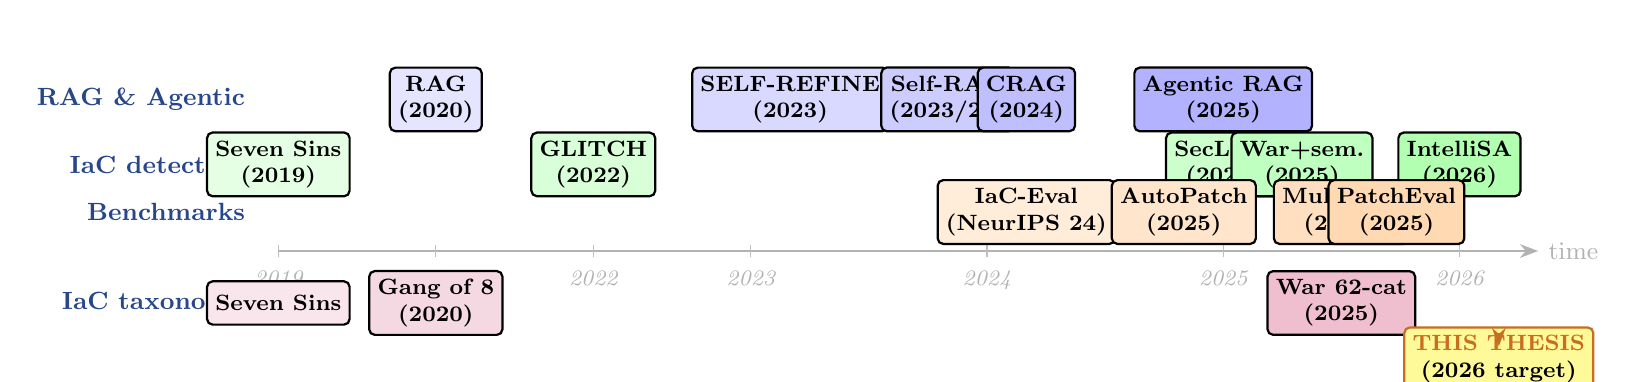
\begin{tikzpicture}[
    yscale=0.55,
    node distance=0.2cm,
    milestone/.style={
      draw, thick, rounded corners=2pt,
      inner sep=3pt, font=\footnotesize\bfseries,
      align=center, minimum height=0.55cm
    },
    track/.style={font=\small\bfseries, anchor=east, text=critblue},
    year/.style={font=\footnotesize\itshape, text=gray!60}
  ]
    % Horizontal time axis
    \draw[-{Stealth[scale=1.0]}, thick, gray!60]
      (0,0) -- (16,0) node[right, font=\small] {time};

    % Year ticks
    \foreach \x/\year in {0/2019, 2/2020, 4/2022, 6/2023, 9/2024, 12/2025, 15/2026} {
      \draw[gray!50] (\x, -0.15) -- (\x, 0.15);
      \node[year, below=0.05cm] at (\x, -0.15) {\year};
    }

    % Track labels on left
    \node[track] at (-0.3, 3.5) {RAG \& Agentic};
    \node[track] at (-0.3, 2.0) {IaC detection};
    \node[track] at (-0.3, 0.9) {Benchmarks};
    \node[track] at (-0.3, -1.2) {IaC taxonomy};

    % RAG track
    \node[milestone, fill=blue!10] at (2, 3.5) {RAG\\(2020)};
    \node[milestone, fill=blue!15] at (6.5, 3.5) {SELF-REFINE\\(2023)};
    \node[milestone, fill=blue!20] at (8.5, 3.5) {Self-RAG\\(2023/24)};
    \node[milestone, fill=blue!25] at (9.5, 3.5) {CRAG\\(2024)};
    \node[milestone, fill=blue!30] at (12, 3.5) {Agentic RAG\\(2025)};

    % IaC detection track
    \node[milestone, fill=green!10] at (0, 2.0) {Seven Sins\\(2019)};
    \node[milestone, fill=green!15] at (4, 2.0) {GLITCH\\(2022)};
    \node[milestone, fill=green!20] at (12, 2.0) {SecLLM\\(2025)};
    \node[milestone, fill=green!25] at (13, 2.0) {War+sem.\\(2025)};
    \node[milestone, fill=green!30] at (15, 2.0) {IntelliSA\\(2026)};

    % Benchmark track
    \node[milestone, fill=orange!15] at (9.5, 0.9) {IaC-Eval\\(NeurIPS 24)};
    \node[milestone, fill=orange!20] at (11.5, 0.9) {AutoPatch\\(2025)};
    \node[milestone, fill=orange!25] at (13.5, 0.9) {Multi-IaC\\(2025)};
    \node[milestone, fill=orange!30] at (14.2, 0.9) {PatchEval\\(2025)};

    % Taxonomy track
    \node[milestone, fill=purple!10] at (0, -1.2) {Seven Sins};
    \node[milestone, fill=purple!15] at (2, -1.2) {Gang of 8\\(2020)};
    \node[milestone, fill=purple!25] at (13.5, -1.2) {War 62-cat\\(2025)};

    % This thesis marker
    \node[milestone, fill=yellow!40, draw=critorange, thick] at (15.5, -2.5)
      {\bfseries\color{critorange} THIS THESIS\\(2026 target)};
    \draw[-{Stealth[scale=1.0]}, thick, critorange]
      (15.5, -1.9) -- (15.5, -2.2);
  \end{tikzpicture}
  }
  \caption{Technology-evolution timeline across four tracks relevant to the
    thesis. The thesis target sits at the intersection of all four --- a
    remediation contribution that uses the 2024-era CRAG retry pattern,
    the 2025 War 62-category taxonomy, and the 2025 PatchEval-style
    scanner-validated evaluation, applied to the IaC domain where
    IntelliSA now sets the 2026 detection baseline.}
  \label{fig:timeline}
\end{figure}

% ============================================================
\chapter{Redirection --- What Rapport 4 Must Contain}
\label{chap:redirection}
% ============================================================

This chapter is the deliverable intent: a blueprint for Rapport~4 and for
the code work that precedes it.

\section{Proposed Rapport~4 structure}

\begin{enumerate}
  \item \textbf{Technology Timeline and Positioning} --- the timeline of
        Chapter~\ref{chap:timeline} and the landscape grid of
        Chapter~\ref{chap:landscape}, with the thesis niche identified.
  \item \textbf{Updated State of the Art} --- add IntelliSA~\citep{intellisa2026},
        PatchEval~\citep{lyu2024patcheval}, AutoPatchBench~\citep{autopatchbench2025},
        SEC-bench~\citep{secbench2025}, SecRepoBench~\citep{secrepobench2025},
        IaC-Eval~\citep{kon2024iaceval}, Multi-IaC-Eval~\citep{multi2025iaceval},
        agentic-RAG survey~\citep{agenticrag2025survey}.
  \item \textbf{Framework (carried over from Rapport~2)} --- no major
        redesign; minor updates to reflect the KICS second-validator
        decision and the self-consistency confidence surrogate.
  \item \textbf{Dataset} --- present the 33{,}667-record corpus
        (Rapport~3) as the primary evaluation dataset; the 8-file suite
        becomes a sanity-check appendix.
  \item \textbf{Evaluation Methodology} --- keep PVR/SER/NNIR; drop the
        log-prob confidence metric; rename the test--retest kappa;
        reduce the ``18 metrics'' count to the actually-computed
        subset.
  \item \textbf{Experimental Results} --- \emph{the critical chapter};
        must report Config~B, C, D on a held-out test split of the 33k
        corpus, with PVR as the headline metric and a direct
        comparison to IntelliSA on the detection layer.
  \item \textbf{Threats to Validity} --- acknowledge LLM non-determinism
        and data leakage; add the KICS/Checkov coverage gap for
        remaining HEURISTIC-only smells.
  \item \textbf{Conclusion and Perspectives}.
\end{enumerate}

\section{Code work to do before Rapport~4}

Ordered by priority:

\begin{enumerate}
  \item \textbf{Finish Phase~4 of the scraping plan} --- Checkov
        validation on the 33k corpus is currently running
        (\texttt{Code/scraping/plan.md}). Needed to populate Tier~A.
  \item \textbf{Add KICS as a second validator} in
        \texttt{Code/src/validator/tool\_integrator.py}. KICS covers
        Ansible/K8s/Docker/CF/Terraform, unlike Checkov's partial
        Ansible support. Closes Issue~3 of
        Chapter~\ref{chap:metrics_audit}.
  \item \textbf{Replace log-prob confidence} in
        \texttt{Code/src/generator/fix\_generator.py} with
        self-consistency confidence over $N=5$ sampled patches. Closes
        Issue~1 of Chapter~\ref{chap:metrics_audit}.
  \item \textbf{Wire the 33k corpus into} \texttt{Code/scripts/evaluate.py}
        as the primary evaluation dataset. Keep the 8-file suite as a
        CI-level unit test.
  \item \textbf{Run Config~B, C, D end-to-end} on the held-out test
        split (3{,}371 records). Collect PVR, SER, NNIR, and the
        detection-layer P/R/F1 comparable to IntelliSA.
  \item \textbf{Reproduce the SOTA baseline} --- run IntelliSA (or its
        nearest public implementation) on the same held-out test split
        so the comparison in Rapport~4 is numerical, not indirect.
\end{enumerate}

\section{Items deliberately left out}

\begin{itemize}
  \item The log-prob confidence Wilcoxon analysis. Not worth salvaging
        on Claude.
  \item The 18-metric framing. Rapport~4 should report the metrics that
        are actually computed, and no others.
  \item OSV/NVD-based Tier~A enrichment --- already determined to be
        low-yield (see the project memory).
\end{itemize}

% ============================================================
\chapter{Summary}
% ============================================================

\begin{gradebox}[Bottom line]{critblue}
Rapport~2 is a solid \emph{design} document and a \emph{plan}. It is not
yet a \emph{results} document. Three of its six claimed contributions do
not survive a careful reading; the other three are defensible but need
empirical backing that does not yet exist. The single most important
missing piece is the Rapport~3 dataset, which is larger than any
comparable IaC smell corpus and should be promoted to the primary
contribution of the thesis. The second most important missing piece is
a Config~D run --- the actual experiment that would justify the
framework's existence. Rapport~4 must deliver both.
\end{gradebox}

The niche is real; the tools to fill it are partly written; the
benchmark landscape has a hole exactly where the thesis aims. What
remains is to run the experiments, report them honestly, and let the
PVR numbers speak.

% ============================================================
\bibliography{references}
\end{document}
